\chapter{Analisis dan Perancangan}
Pada bab ini dijelaskan analisis terkait kebutuhan sistem pada KodeBareng, masalah pada implementasi ILE yang sudah ada, serta rancangan solusi yang akan diimplementasikan.

\section{Analisis Masalah}

Kompleksitas dari pemrograman itu sendiri menyebabkan sulitnya pelajar yang baru mempelajari pemrograman memahami konsep-konsep dan abstrak dari pemrograman \parencite{moons2013pilot}. Kurangnya kemampuan dalam menelusuri jejak suatu kode program, serta belum terbentuknya model kerangka pikir terhadap cara program komputer bekerja \parencite{mayer1981psychology} merupakan faktor-faktor yang membuat pelajar tidak dapat menyerap informasi teknis baru terkait pemrograman dengan maksimal. Maka dari itu, diperlukan suatu bentuk model konkret terkait alur proses kerja suatu program komputer sehingga dapat mempermudah proses transfer ilmu konsep-konsep pemrograman kepada pelajar. Pembelajaran interaktif menjadi salah satu cara yang dapat dimanfaatkan karena dapat diaplikasikan secara daring menggunakan teknologi digital yang sudah tersedia.

Menurut \textcite{moons2013pilot}, terdapat 4 pendekatan yang dapat dilakukan untuk memecahkan masalah tersebut. Pendekatan pertama adalah dengan menggunakan urutan paradigma pemrograman tertentu dalam pembelajarannya sehingga konsep-konsep yang lebih dalam pada pemrograman tidak harus dipelajari dari awal. Pendekatan kedua adalah dengan menggunakan teknik pembelajaran secara aktif, seperti lokakarya dan penceritaan dengan narasi. Namun, pendekatan ini agak sulit diaplikasikan pada pembelajaran secara daring. Pendekatan ketiga adalah dengan menggunakan bahasa pemrograman yang lebih sesuai untuk pelajar pemrograman, seperti Python dan Eiffel. Pendekatan keempat adalah menggunakan lingkungan pembelajaran interaktif atau \textit{interactive learning environment} (ILE) yang dapat berbentuk \textit{microworld}, visualisasi algoritma, dan visualisasi eksekusi program.

Karena pembelajaran interaktif pada KodeBareng masih hanya sebatas pembawaan materi, pengalaman pembelajarannya masih dianggap kurang interaktif dan sama dengan platform kelas pembelajaran pemrograman lainnya seperti yang telah dibahas pada \autoref{sssec:ragam-implementasi-ile}. Maka dari itu, dibutuhkan suatu \textit{interactive learning environment} (ILE) yang dapat mendukung pembelajaran interaktif dan memecahkan masalah sulitnya mempelajari pemrograman bagi orang yang baru mempelajari pemrograman. ILE dikembangkan menggunakan pendekatan \textcite{moons2013pilot} sehingga dapat meningkatkan pemahaman konsep serta mendukung pemrograman praktis pelajar sesuai dengan komponen penting pembelajaran pemrograman secara daring menurut \textcite{choy2004interactive}. ILE dibangun secara modular pada platform KodeBareng sehingga tidak terlalu disruptif terhadap sistem yang sudah ada.

Perbandingan aspek fitur KodeBareng dengan beberapa platform lainnya dapat dilihat pada \autoref{tab:platform-comparison}. Berdasarkan perbandingan tersebut, visualisasi eksekusi kode yang merupakan pendekatan keempat dari \textcite{moons2013pilot} menjadi salah satu aspek yang menarik karena tidak banyak ditemukan implementasinya pada platform kelas pembelajaran pemrograman yang sudah ada. Hal ini akan menjadi keunikan tersendiri karena berbeda dari platform kelas pembelajaran pemrograman lainnya sehingga dapat menjadi nilai tambah pada platform pembelajaran pemrograman KodeBareng.

\small
\begin{longtable}[c]{|>{\raggedright\arraybackslash\setlength{\baselineskip}{0.75\baselineskip}}p{0.2\linewidth}|l|l|l|>{\raggedright\arraybackslash\setlength{\baselineskip}{0.75\baselineskip}}p{0.15\linewidth}|>{\raggedright\arraybackslash\setlength{\baselineskip}{0.75\baselineskip}}p{0.15\linewidth}|}
  \caption{Perbandingan fitur KodeBareng dengan platform yang sudah ada} \label{tab:platform-comparison}                                                                                                                                                                                                                                                                                                                                                                                                                                                                                          \\ \hline
  \rowcolor[HTML]{C0C0C0}
  \multicolumn{1}{|c|}{\cellcolor[HTML]{C0C0C0}\textbf{Aspek}} & \multicolumn{1}{c|}{\cellcolor[HTML]{C0C0C0}\textbf{Sololearn}} & \multicolumn{1}{c|}{\cellcolor[HTML]{C0C0C0}\textbf{Brilliant}} & \multicolumn{1}{c|}{\cellcolor[HTML]{C0C0C0}\textbf{Progate}} & \multicolumn{1}{>{\centering\arraybackslash\setlength{\baselineskip}{0.75\baselineskip}}p{0.15\linewidth}|}{\cellcolor[HTML]{C0C0C0}\textbf{Python Tutor}} & \multicolumn{1}{>{\centering\arraybackslash\setlength{\baselineskip}{0.75\baselineskip}}p{0.15\linewidth}|}{\cellcolor[HTML]{C0C0C0}\textbf{KodeBareng (awal)}} \\ \hline
  \endfirsthead
  %
  \caption*{\autoref{tab:platform-comparison} (lanjutan): Perbandingan fitur KodeBareng dengan platform yang sudah ada}                                                                                                                                                                                                                                                                                                                                                                                                                                                                           \\ \hline
  \rowcolor[HTML]{C0C0C0}
  \multicolumn{1}{|c|}{\cellcolor[HTML]{C0C0C0}\textbf{Aspek}} & \multicolumn{1}{c|}{\cellcolor[HTML]{C0C0C0}\textbf{Sololearn}} & \multicolumn{1}{c|}{\cellcolor[HTML]{C0C0C0}\textbf{Brilliant}} & \multicolumn{1}{c|}{\cellcolor[HTML]{C0C0C0}\textbf{Progate}} & \multicolumn{1}{>{\centering\arraybackslash\setlength{\baselineskip}{0.75\baselineskip}}p{0.15\linewidth}|}{\cellcolor[HTML]{C0C0C0}\textbf{Python Tutor}} & \multicolumn{1}{>{\centering\arraybackslash\setlength{\baselineskip}{0.75\baselineskip}}p{0.15\linewidth}|}{\cellcolor[HTML]{C0C0C0}\textbf{KodeBareng (awal)}} \\ \hline
  \endhead
  %
  Kelas pemrograman                                            & Ada                                                             & Ada                                                             & Ada                                                           & Tidak ada                                                                                                                                                  & Ada                                                                                                                                                             \\ \hline
  Pembawaan materi interaktif                                  & Tidak ada                                                       & Ada                                                             & Ada                                                           & Tidak ada                                                                                                                                                  & Ada                                                                                                                                                             \\ \hline
  Latihan soal kode                                            & Ada                                                             & Tidak ada                                                       & Ada                                                           & Tidak ada                                                                                                                                                  & Ada                                                                                                                                                             \\ \hline
  Visualisasi eksekusi kode                                    & Tidak ada                                                       & Tidak ada                                                       & Tidak ada                                                     & Ada                                                                                                                                                        & Tidak ada                                                                                                                                                       \\ \hline
\end{longtable}
\normalsize

ILE berupa kakas visualisasi eksekusi kode juga dapat digunakan untuk menanamkan model konkret kerangka pikir terhadap cara komputer bekerja \parencite{mayer1981psychology} dan juga dapat membantu pelajar dalam menelusuri alur kerja program komputer. Dengan visualisasi eksekusi kode, pelajar dapat mengeksplorasi ILE tersebut sehingga dapat membangun pemahaman konsep kerja program dengan pemikiran masing-masing dan membuat pembelajaran interaktif di KodeBareng menggunakan pendekatan kedua yaitu belajar "dengan" pembelajaran interaktif yang lebih efektif \parencite{reeves2012interactive}. Visualisasi eksekusi kode juga dapat meningkatkan dukungan terhadap aktivitas pemrograman secara praktis \parencite{choy2004interactive} sehingga meningkatkan dukungan pembelajaran pemrograman secara daring pada KodeBareng. Visualisasi eksekusi kode dapat diintegrasikan di KodeBareng pada modul materi pembelajaran sesuai dengan saran letak pemberian model konkret menurut \textcite{mayer1981psychology} serta pada latihan soal pemrograman seperti pada penelitian \textcite{moons2013pilot}.

\section{Analisis Kebutuhan} \label{sec:analisis-kebutuhan}
Seperti yang sudah dijelaskan pada Bab sebelumnya, KodeBareng merupakan platform web pembelajaran pemrograman yang ingin membawakan pembelajarannya secara visual dan interaktif. Berdasarkan analisis masalah, pendekatan yang akan dipilih adalah dengan membuat ILE berupa visualisasi eksekusi kode yang akan diintegrasikan pada platform web KodeBareng. ILE tersebut dapat memvisualisasikan eksekusi kode yang diberikan sehingga dapat memberikan gambaran mengenai bagaimana alur cara suatu kode program bekerja. Berbeda dengan platform lainnya yang mendukung interaktivitasnya dengan adanya animasi visual ataupun Web IDE yang dapat mengeksekusi program secara langsung, pendekatan dengan menggunakan visualisasi eksekusi kode dapat diintegrasikan dengan pembawaan materi pembelajaran serta pengerjaan latihan soal sehingga dapat mencapai tujuannya yaitu meningkatkan pemahaman orang yang baru mempelajari pemrograman dengan memberikan model kerangka eksekusi kode yang dapat dieksplorasi menggunakan kodenya sendiri. Pendekatan ini sesuai dengan yang dilakukan oleh \textcite{moons2013pilot} dan \textcite{mayer1981psychology}.

Maka dari itu, dirancanglah diagram \textit{use case} baru yang sesuai dengan kebutuhan dan pendekatan terkait yang dapat dilihat pada \autoref{fig:diagram-usecase-v2}. Penjelasan terkait \textit{use case} tersebut dapat dilihat pada \autoref{tab:exp-diagram-usecase-v2}.

\begin{figure}[!h]
  \centering
  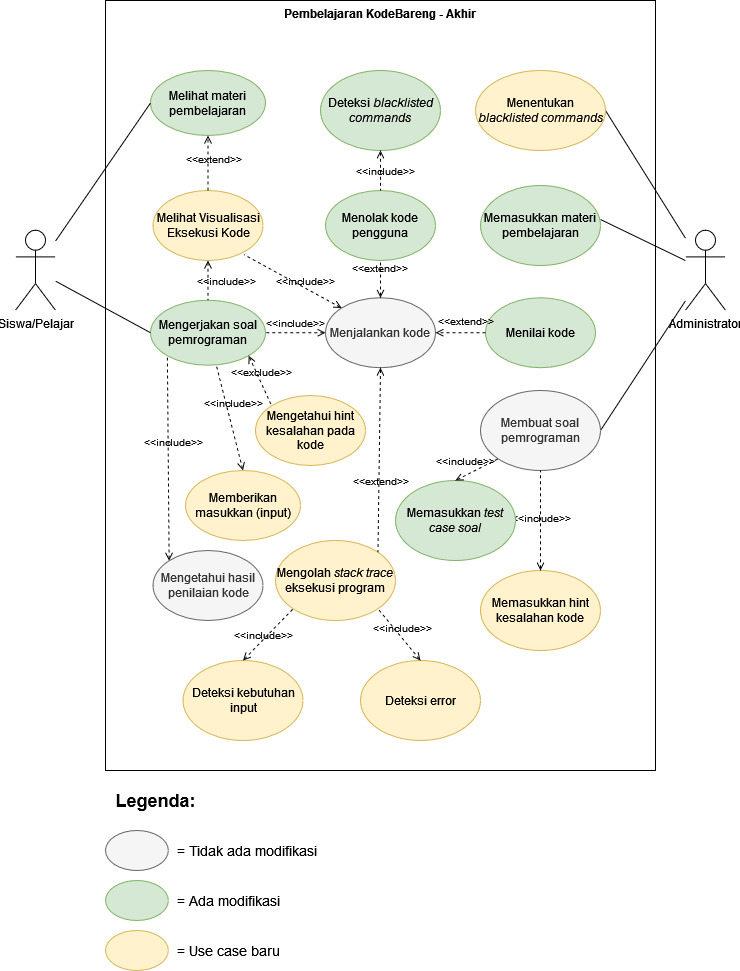
\includegraphics[width=1.15\textwidth]{chapter3/diagram_usecase_v2.jpg}
  \caption{\textit{Use Case} pembelajaran pemrograman KodeBareng setelah perubahan} \label{fig:diagram-usecase-v2}
  Sumber: Penulis (2022)
\end{figure}

\small
\begin{longtable}[c]{|l|>{\setlength{\baselineskip}{0.75\baselineskip}}p{0.3\linewidth}|>{\setlength{\baselineskip}{0.75\baselineskip}}p{0.5\linewidth}|}
  \caption{Penjelasan \textit{Use Case} pembelajaran pemrograman KodeBareng setelah perubahan} \label{tab:exp-diagram-usecase-v2}                                                                                                                                                                                                                    \\ \hline
  \rowcolor{gray!30}
  \textbf{ID} & \textbf{Kebutuhan}                             & \textbf{Penjelasan}                                                                                                                                                                                                                                                                 \\ \hline
  \endfirsthead
  %
  \caption*{\autoref{tab:exp-diagram-usecase-v2} (lanjutan): Penjelasan \textit{Use Case} pembelajaran pemrograman KodeBareng setelah perubahan}                                                                                                                                                                                                     \\ \hline
  \rowcolor{gray!30}
  \textbf{ID} & \textbf{Kebutuhan}                             & \textbf{Penjelasan}                                                                                                                                                                                                                                                                 \\ \hline
  \endhead
  %
  UC-01       & Melihat materi pembelajaran                    & Pelajar dapat melihat materi pembelajaran berupa teks dan gambar. Perubahannya adalah integrasi ILE  sehingga pada materi dapat dimasukkan visualisasi eksekusi kode.                                                                                                               \\ \hline
  UC-02       & Mengerjakan soal pemrograman                   & Pelajar dapat mengerjakan latihan soal pemrograman. Perubahannya adalah soal pemrograman kini dilengkapi ILE yang dapat memvisualisasikan eksekusi kode serta memberikan hint apabila ada kesalahan dalam mengerjakan soal.                                                         \\ \hline
  UC-03       & Melihat visualisasi eksekusi kode              & Pelajar dapat melihat visualisasi kode berupa alur kerja eksekusi program serta data-data apa saja yang terdapat dalam memori.                                                                                                                                                      \\ \hline
  UC-04       & Mengetahui hasil penilaian kode                & Pelajar dapat mengetahui kebenaran dari kode yang dimasukkan pada latihan pemrograman.                                                                                                                                                                                              \\ \hline
  UC-05       & Memberikan masukkan (input)                    & Pelajar dapat memberikan input yang akan dimasukkan pada kode yang akan dieksekusi.                                                                                                                                                                                                 \\ \hline
  UC-06       & Mengetahui hint kesalahan pada kode            & Pelajar dapat melihat hint kesalahan apabila kode yang dimasukkan pada latihan pemrograman salah.                                                                                                                                                                                   \\ \hline
  UC-07       & Menjalankan kode                               & Pelajar dapat menjalankan kode yang dimasukkan serta melihat keluarannya.                                                                                                                                                                                                           \\ \hline
  UC-08       & Menolak kode pelajar                           & Kode yang dimasukkan oleh pelajar dapat ditolak oleh sistem apabila tidak sesuai dengan batasan-batasan perintah yang dapat dieksekusi oleh ILE. Perubahannya adalah batasan eksekusi program dapat ditentukan oleh administrator (sebelumnya ditentukan secara \textit{hard code}) \\ \hline
  UC-09       & Deteksi \textit{blacklisted commands}          & Sistem memiliki daftar perintah yang tidak boleh dieksekusi agar tidak mengancam keamanan sistem. Perubahannya adalah perintah yang dieksekusi kini bersifat dinamis tergantung pada definisi yang diberikan oleh Administrator.                                                    \\ \hline
  UC-11       & Menilai kode                                   & Sistem dapat menilai kode yang dijalankan secara \textit{blackbox autograding}. Perubahannya adalah penilaian kini dapat menggunakan lebih dari satu \textit{test case} serta dapat menerima \textit{input}.                                                                        \\ \hline
  UC-12       & Mengolah \textit{stack trace} eksekusi program & Sistem dapat mengolah \textit{stack trace} dari program yang dieksekusi agar dapat memperoleh informasi alur kerja dan data selama eksekusi program.                                                                                                                                \\ \hline
  UC-13       & Deteksi kebutuhan input                        & Sistem dapat mendeteksi jika kode program membutuhkan input untuk melanjutkan eksekusinya.                                                                                                                                                                                          \\ \hline
  UC-14       & Deteksi error                                  & Sistem dapat mendeteksi error pada eksekusi program.                                                                                                                                                                                                                                \\ \hline
  UC-15       & Menentukan \textit{blacklisted commands}       & Administrator dapat menentukan perintah-perintah yang tidak boleh dieksekusi pada kode program.                                                                                                                                                                                     \\ \hline
  UC-16       & Memasukkan materi pembelajaran                 & Administrator dapat memasukkan penjelasan materi pada modul-modul kelas pembelajaran. Perubahannya adalah Administrator dapat menambahkan visualisasi eksekusi kode dalam penjelasan materi.                                                                                        \\ \hline
  UC-17       & Membuat soal pemrograman                       & Administrator dapat membuat soal pemrograman.                                                                                                                                                                                                                                       \\ \hline
  UC-18       & Memasukkan \textit{test case} soal             & Administrator dapat memasukkan \textit{test case} penilaian pada suatu soal. Perubahannya adalah \textit{test case} yang dimasukkan bisa memiliki input.                                                                                                                            \\ \hline
  UC-19       & Memasukkan hint kesalahan kode                 & Administrator dapat menentukan hint kesalahan yang ditampilkan pada suatu soal.                                                                                                                                                                                                     \\ \hline
\end{longtable}
\normalsize

Berdasarkan \textit{use case} baru yang telah dibuat pada \autoref{fig:diagram-usecase-v2}, diturunkanlah spesifikasi kebutuhan perangkat lunak fungsional dan non-fungsional yang dapat dilihat pada \autoref{tab:srs-fungsional} dan \autoref{tab:srs-nonfungsional}.

Spesifikasi fungsional menjelaskan fungsi-fungsi yang dapat dijalankan pada ILE yang akan dibuat. Spesifikasi ini diturunkan dari diagram \textit{use case} sesuai dengan siapa dan apa yang dapat dilakukan. Penjelasan lebih detail mengenai spesifikasi fungsional dapat dilihat pada \autoref{tab:srs-fungsional}.

\small
\begin{longtable}[c]{|l|>{\setlength{\baselineskip}{0.75\baselineskip}}p{0.5\linewidth}|>{\setlength{\baselineskip}{0.75\baselineskip}}p{0.3\linewidth}|}
  \caption{Spesifikasi kebutuhan fungsional ILE KodeBareng} \label{tab:srs-fungsional}                                                                                                                                                                                   \\ \hline
  \rowcolor{gray!30}
  \textbf{ID} & \textbf{Kebutuhan}                                                                      & \textbf{Penjelasan}                                                                                                                                            \\ \hline
  \endfirsthead
  %
  \caption*{\autoref{tab:srs-fungsional} (lanjutan): Spesifikasi kebutuhan fungsional ILE KodeBareng}                                                                                                                                                                    \\ \hline
  \rowcolor{gray!30}
  \textbf{ID} & \textbf{Kebutuhan}                                                                      & \textbf{Penjelasan}                                                                                                                                            \\ \hline
  \endhead
  %
  KB-F-01     & Pelajar memasukkan kode program pada sistem                                             & Menggunakan kakas Monaco Editor.                                                                                                                               \\ \hline
  KB-F-02     & Pelajar memasukkan input program pada sistem                                            & Masukan diminta apabila kode membutuhkan masukan.                                                                                                              \\ \hline
  KB-F-03     & Pelajar dapat menjalankan kode                                                          & Pelajar dapat melihat hasil eksekusi kode.                                                                                                                     \\ \hline
  KB-F-04     & Pelajar dapat melihat hasil visualisasi eksekusi kode                                   & Pelajar dapat melihat perubahan data dan \textit{flow} program yang dijalankan. Pelajar juga dapat mengeksplorasi langkah-langkah eksekusi.                    \\ \hline
  KB-F-05     & Pelajar mendapat penilaian dari hasil eksekusi kode                                     & Penilaian berdasarkan teknik \textit{blackbox autograding}.                                                                                                    \\ \hline
  KB-F-06     & Pelajar mendapat \textit{hint} kesalahan pada kode program                              & -                                                                                                                                                              \\ \hline
  KB-F-07     & Pelajar dapat melihat pesan error pada program                                          & -                                                                                                                                                              \\ \hline
  KB-F-08     & Sistem menolak kode pelajar apabila terdapat perintah-perintah yang tidak diperbolehkan & Keterbatasan eksekusi ditentukan oleh Administrator.                                                                                                           \\ \hline
  KB-F-09     & Sistem menilai kode program menggunakan \textit{test case}                              & -                                                                                                                                                              \\ \hline
  KB-F-10     & Sistem mengolah \textit{stack trace} eksekusi program                                   & \textit{Stack trace} berisi daftar fungsi, variabel, modul, serta \textit{stack frame} pada tiap langkah eksekusi program. Debugger yang digunakan adalah pdb. \\ \hline
  KB-F-11     & Administrator menentukan perintah-perintah yang tidak diperbolehkan                     & -                                                                                                                                                              \\ \hline
  KB-F-12     & Administrator memasukkan konten materi pembelajaran                                     & Dapat memasukkan visualisasi kode pada materi pembelajaran.                                                                                                    \\ \hline
  KB-F-13     & Administrator membuat soal pemrograman                                                  & -                                                                                                                                                              \\ \hline
  KB-F-14     & Administrator memasukkan \textit{test case} soal pemrograman                            &                                                                                                                                                                \\ \hline
  KB-F-15     & Administrator memasukkan \textit{hint} kesalahan yang dapat ditampilkan pada soal       & -                                                                                                                                                              \\ \hline
\end{longtable}
\normalsize

Spesifikasi non-fungsional diturunkan dari kebutuhan KodeBareng agar tujuan dapat tercapai dan sistem berjalan dengan lancar. Maka dari itu, diturunkanlah spesifikasi berupa batasan respon hasil eksekusi agar pelajar tidak terlalu lama menunggu hasil eksekusi, desain sistem yang memudahkan dilakukan pengetesan terhadap berbagai macam kode, serta membatasi apa yang dapat dieksekusi agar keamanan sistem dapat terjaga. Penjelasan lebih detail mengenai spesifikasi fungsional dapat dilihat pada \autoref{tab:srs-nonfungsional}.

\small
\begin{longtable}[c]{|l|l|>{\setlength{\baselineskip}{0.75\baselineskip}}p{0.6\linewidth}|}
  \caption{Spesifikasi kebutuhan non-fungsional ILE KodeBareng} \label{tab:srs-nonfungsional}                \\ \hline
  \rowcolor{gray!30}
  \textbf{ID} & \textbf{Parameter} & \textbf{Kebutuhan}                                                      \\ \hline
  \endfirsthead
  %
  \caption*{\autoref{tab:srs-nonfungsional} (lanjutan): Spesifikasi kebutuhan non-fungsional ILE KodeBareng} \\ \hline
  \rowcolor{gray!30}
  \textbf{ID} & \textbf{Parameter} & \textbf{Kebutuhan}                                                      \\ \hline
  \endhead
  %
  KB-NF-01    & Performance        & Sistem mengembalikan hasil eksekusi paling lama 10 detik.               \\ \hline
  KB-NF-02    & Testability        & Sistem dirancang sedemikian rupa sehingga mudah dilakukan pengetesan.   \\ \hline
  KB-NF-03    & Security           & Sistem tidak membiarkan terjadinya eksekusi kode berbahaya.             \\ \hline
\end{longtable}
\normalsize

Pemetaan hasil penurunan antara \textit{use case} dengan spesifikasi kebutuhan terkait dapat dilihat pada \autoref{tab:srs-usecase}.

\small
\begin{longtable}[c]{|l|>{\setlength{\baselineskip}{0.75\baselineskip}}p{0.5\linewidth}|}
  \caption{Keterkaitan SRS dan Use Case} \label{tab:srs-usecase}                \\ \hline
  \rowcolor{gray!30}
  \textbf{ID SRS} & \textbf{ID Use Case}                                        \\ \hline
  \endfirsthead
  %
  \caption*{\autoref{tab:srs-usecase} (lanjutan): Keterkaitan SRS dan Use Case} \\ \hline
  \rowcolor{gray!30}
  \textbf{ID SRS} & \textbf{ID Use Case}                                        \\ \hline
  \endhead
  %
  KB-F-01         & UC-02                                                       \\ \hline
  KB-F-02         & UC-05, UC-13                                                \\ \hline
  KB-F-03         & UC-02, UC-04, UC-07                                         \\ \hline
  KB-F-04         & UC-01, UC-02, UC-03                                         \\ \hline
  KB-F-05         & UC-04, UC-11                                                \\ \hline
  KB-F-06         & UC-06                                                       \\ \hline
  KB-F-07         & UC-02, UC-14                                                \\ \hline
  KB-F-08         & UC-08, UC-09                                                \\ \hline
  KB-F-09         & UC-11                                                       \\ \hline
  KB-F-10         & UC-12                                                       \\ \hline
  KB-F-11         & UC-15                                                       \\ \hline
  KB-F-12         & UC-16                                                       \\ \hline
  KB-F-13         & UC-17                                                       \\ \hline
  KB-F-14         & UC-18                                                       \\ \hline
  KB-F-15         & UC-19                                                       \\ \hline
\end{longtable}
\normalsize

\section{Rancangan Solusi}

Berdasarkan hasil analisis permasalahan dan kebutuhan sebelumnya, dibuatlah rancangan komponen implementasi pada subsistem-subsistem yang terdapat pada KodeBareng. Rancangan tersebut berupa diagram komponen yang terdapat pada \autoref{fig:diagram-komponen}. Rancangan ini menggambarkan komponen apa saja yang akan dimodifikasi ataupun ditambahkan pada sistem KodeBareng terkait pembelajaran pemrograman yang sudah ada.

\begin{figure}[!h]
  \centering
  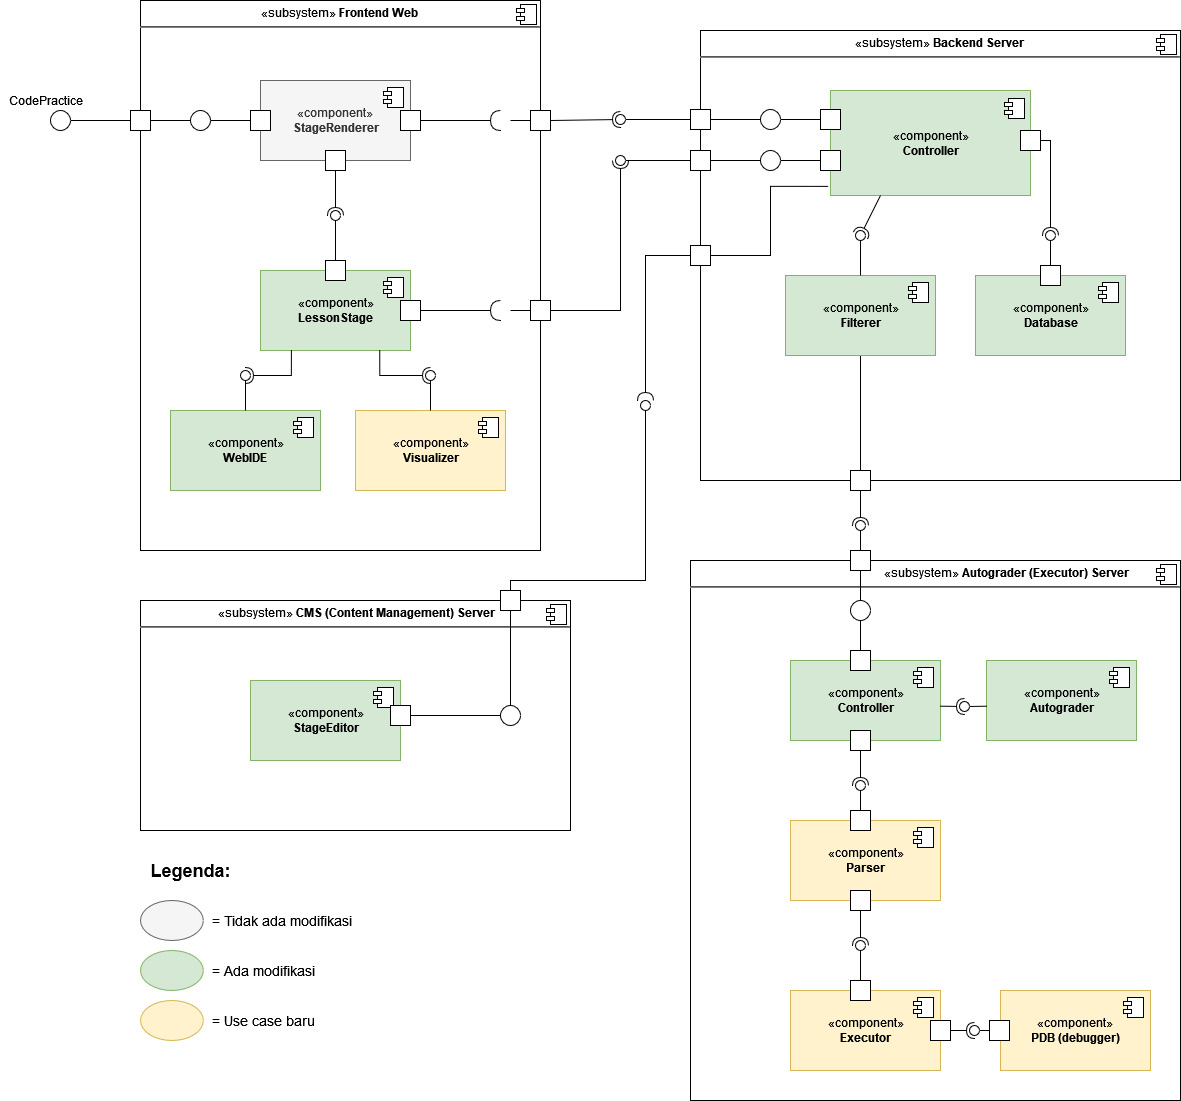
\includegraphics[width=1.1\textwidth]{chapter3/diagram_komponen.jpg}
  \caption{Diagram komponen} \label{fig:diagram-komponen}
  Sumber: Penulis (2022)
\end{figure}

ILE akan diintegrasikan pada komponen-komponen terkait materi pembelajaran di KodeBareng. Maka dari itu, komponen-komponen yang akan dimodifikasi atau ditambahkan akan terkait dengan komponen Stage yang mendefinisikan bagaimana suatu tahap (\textit{stage}) materi pada suatu modul pembelajaran dijelaskan (berupa teks, latihan pemrograman, dsb). Alur pembelajaran pelajar dapat dilihat pada \autoref{fig:activity-overall}.

\begin{figure}[!h]
  \centering
  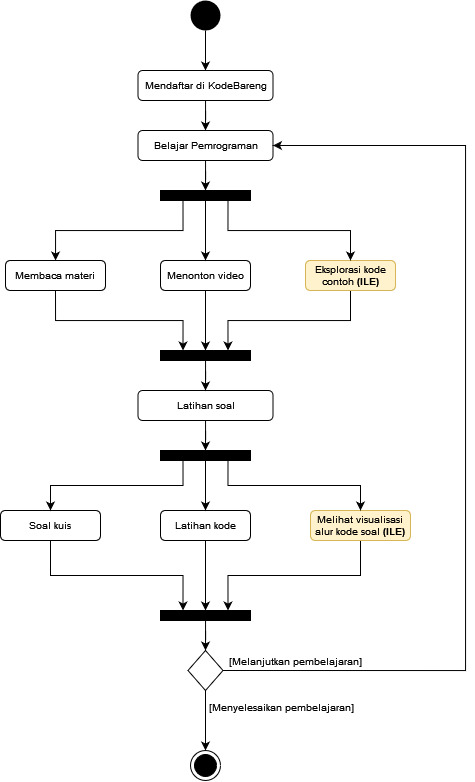
\includegraphics[width=0.85\textwidth]{chapter3/activity-overall.jpg}
  \caption{Activity Diagram Pelajar} \label{fig:activity-overall}
  Sumber: Penulis (2022)
\end{figure}

Alur program utama terkait visualisasi eksekusi kode dimulai dari pelajar atau sistem memasukkan kode pada Web IDE yang digunakan pada sistem \textit{Frontend}, kemudian melakukan permintaan kepada sistem \textit{Backend} untuk memvisualisasikan kode tersebut. Sistem \textit{Backend} akan memfilter kode yang akan dieksekusi, lalu apabila lolos akan dilanjutkan kepada sistem \textit{Autograder-Executor} untuk mendapatkan hasil olahan eksekusi program yang dapat divisualisasikan. Hasil tersebut dikembalikan pada sistem \textit{Frontend} untuk divisualisasikan dan dieksplorasi langkah-langkah eksekusinya oleh pelajar. Pada \autoref{fig:activity-ile} dapat dilihat alur program utama ketika dijalankan oleh pelajar.

\begin{figure}[!h]
  \centering
  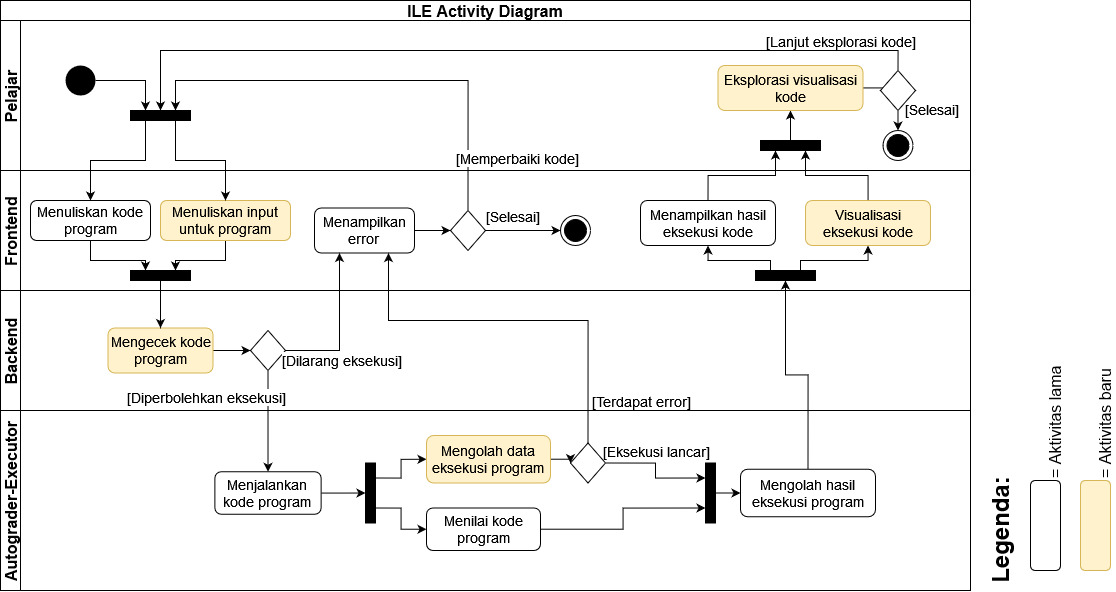
\includegraphics[width=1.6\textwidth, angle=-90]{chapter3/activity-ile.jpg}
  \caption{Activity Diagram ILE} \label{fig:activity-ile}
  Sumber: Penulis (2022)
\end{figure}

Pada sistem \textit{Frontend}, ditambahkan komponen baru yaitu Visualizer yang dapat memvisualisasikan kode eksekusi yang dimasukkan pada komponen Web IDE. Web IDE yang sudah ada dimodifikasi sehingga dapat berinteraksi dengan Visualizer serta dapat memiliki mode latihan soal atau materi sehingga dapat dipakai pada penjelasan materi (tanpa penilaian) dan latihan soal (dengan penilaian). Visualizer harus dapat menampilkan isi dari suatu program saat dijalankan pada tiap langkah eksekusinya, seperti baris kode yang sedang dieksekusi, isi dari variabel-variabel yang terdapat dalam memori \textit{runtime} program, hasil keluaran program, serta pesan \textit{error} yang terjadi. Visualizer dapat dieksplorasi oleh pengguna dengan cara mengubah input yang dimasukkan pada program yang dijalankan, mengubah kode program yang ingin divisualisasikan, serta dapat melihat alur eksekusi kode program secara maju ataupun mundur yang dapat dikontrol oleh pengguna. Gambaran desain \textit{low-fidelity} dari komponen Visualizer dapat dilihat pada \autoref{fig:wireframe-explanation}, \autoref{fig:wireframe-quiz}, dan \autoref{fig:wireframe-lesson}.

\begin{figure}[!h]
  \centering
  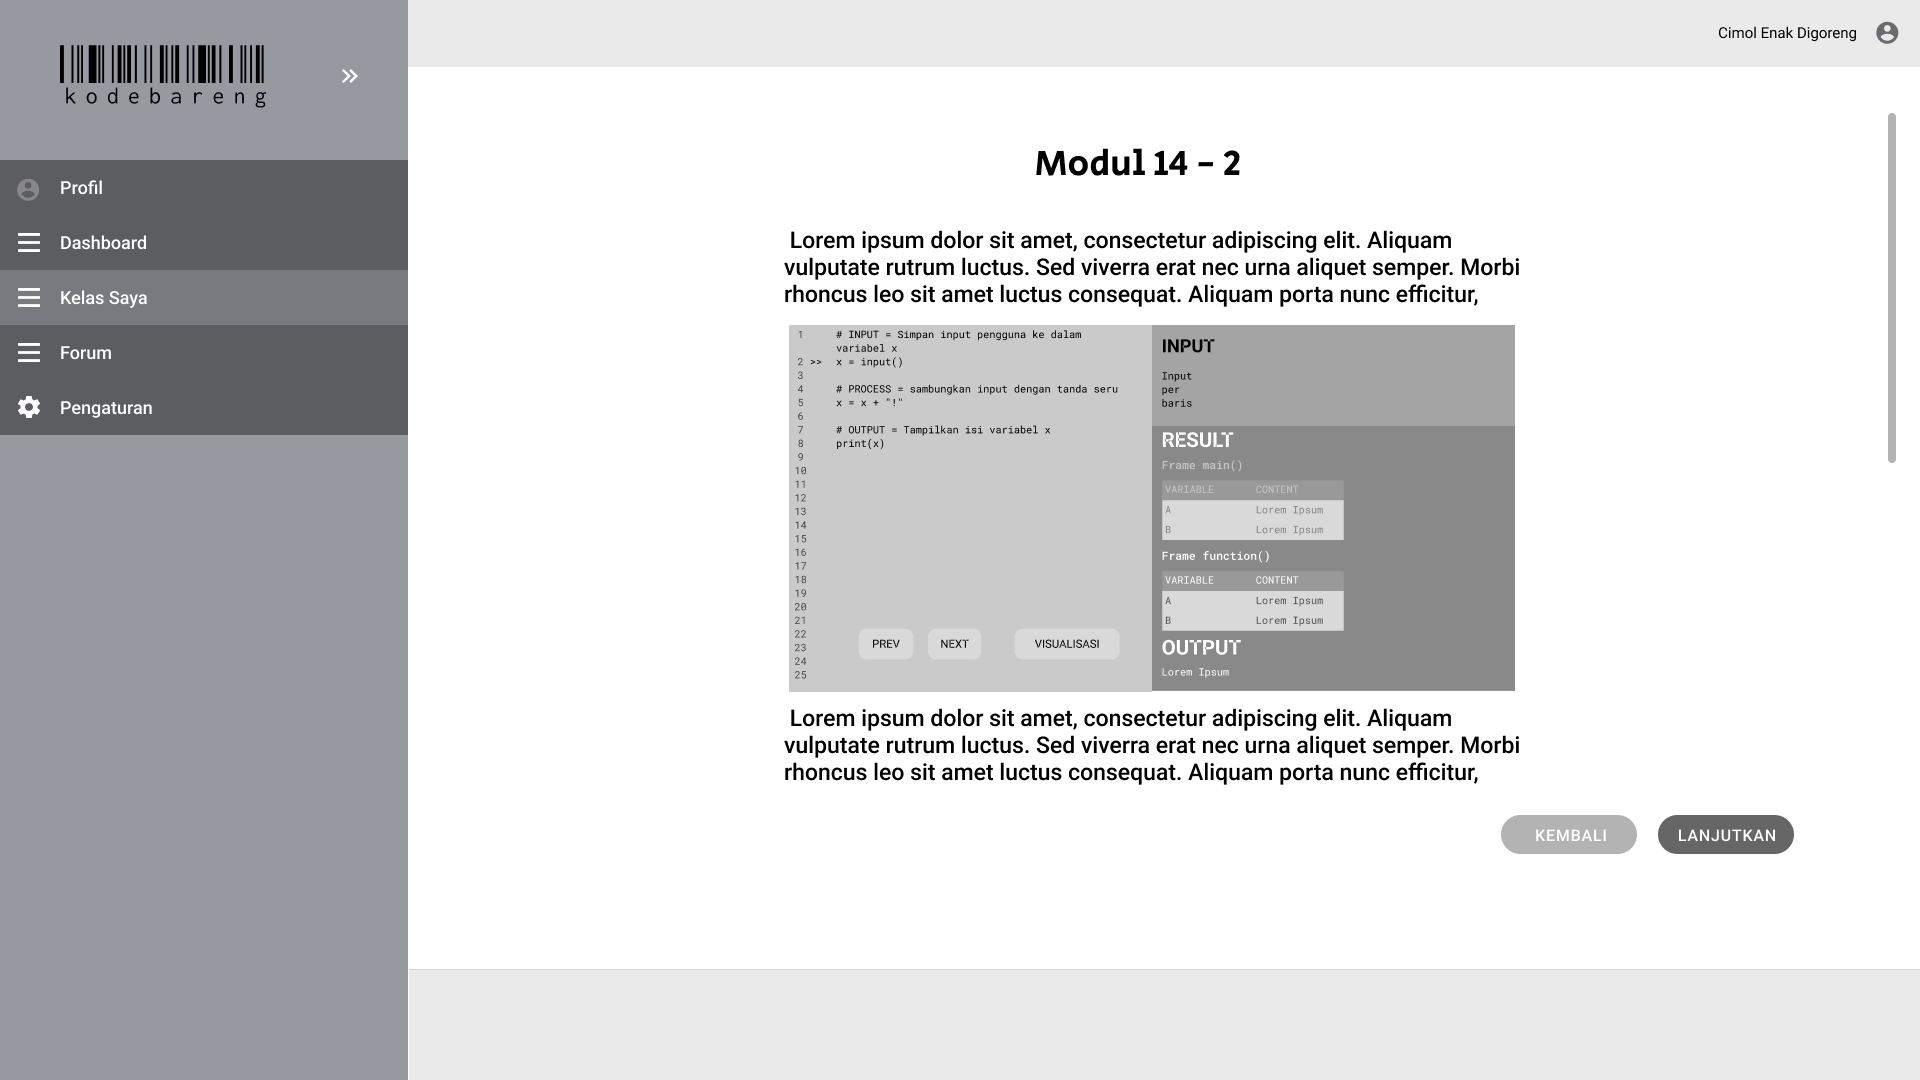
\includegraphics[width=\textwidth]{chapter3/visualizer-explanation.png}
  \caption{Wireframe Visualizer pada Explanation Stage} \label{fig:wireframe-explanation}
  Sumber: Penulis (2022)
\end{figure}

\begin{figure}[!h]
  \centering
  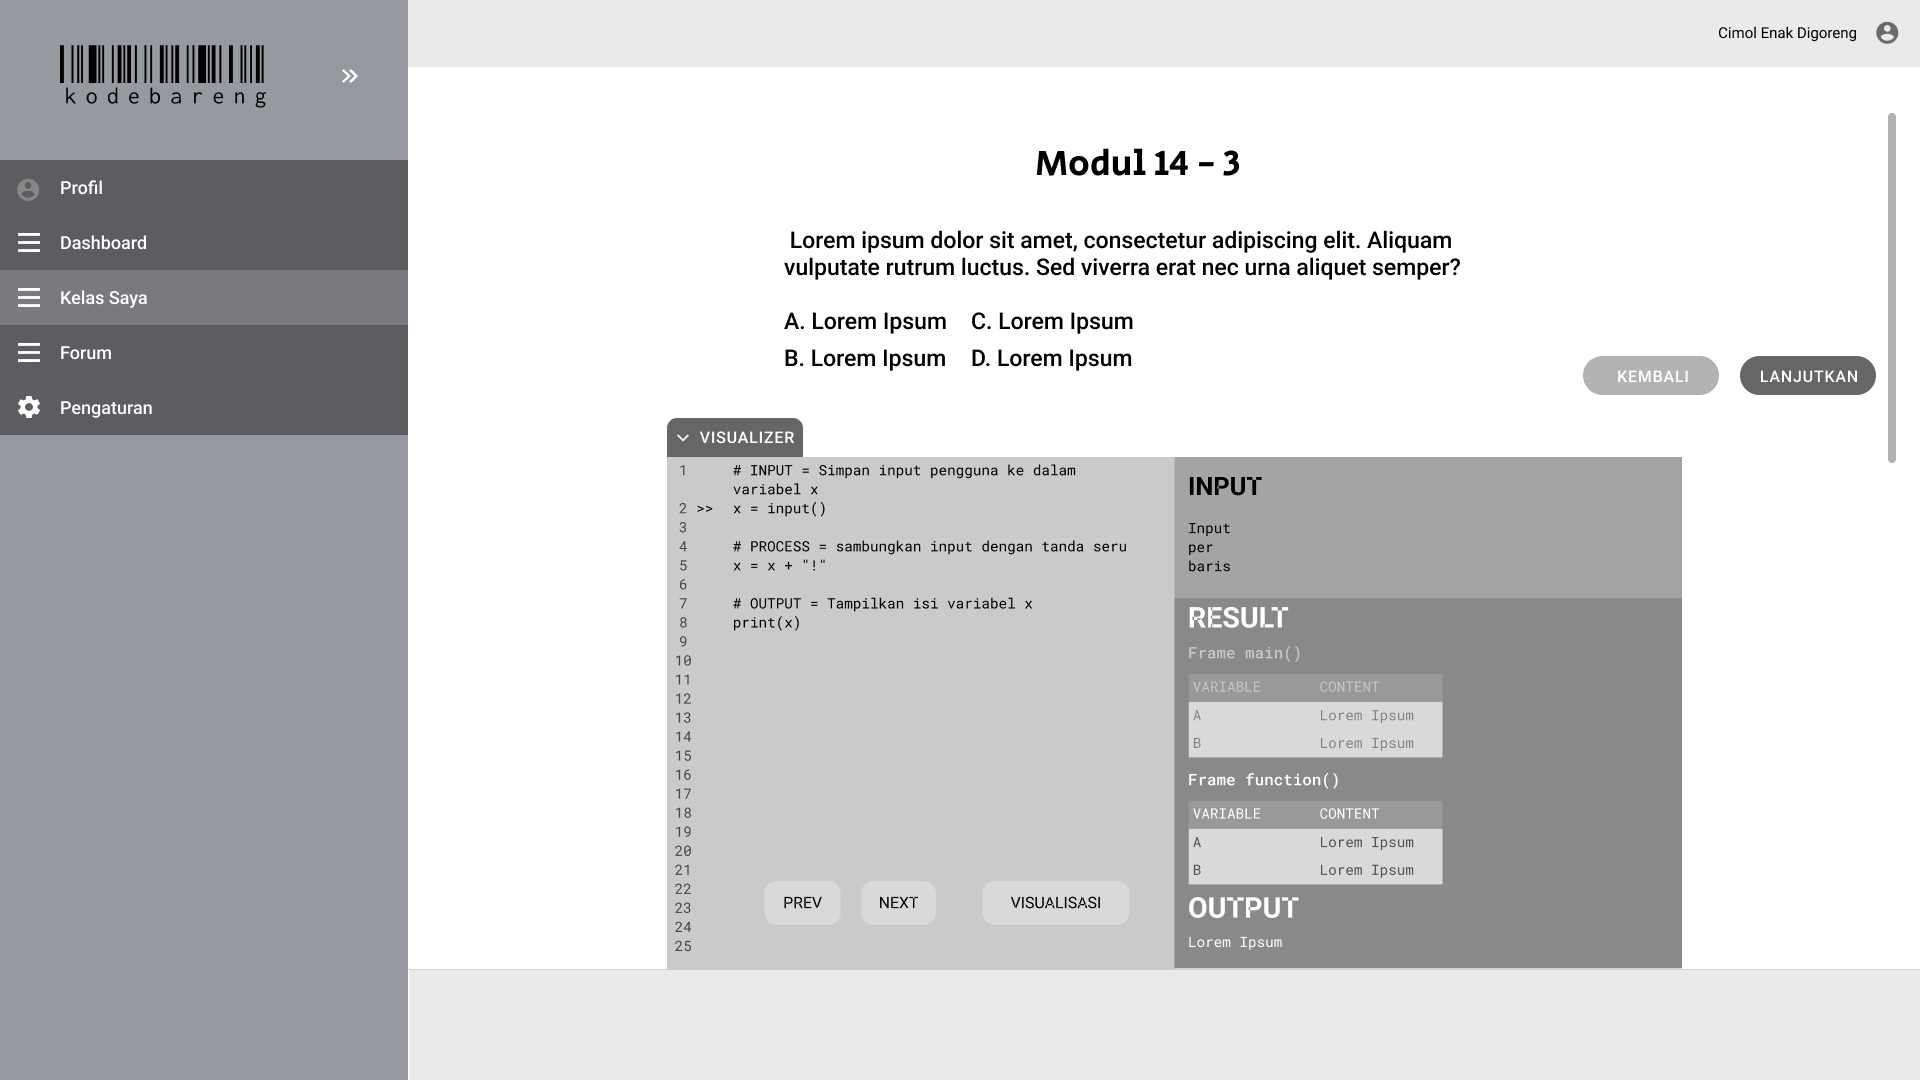
\includegraphics[width=\textwidth]{chapter3/visualizer-quiz.png}
  \caption{Wireframe Visualizer pada Quiz Stage} \label{fig:wireframe-quiz}
  Sumber: Penulis (2022)
\end{figure}

\begin{figure}[!h]
  \centering
  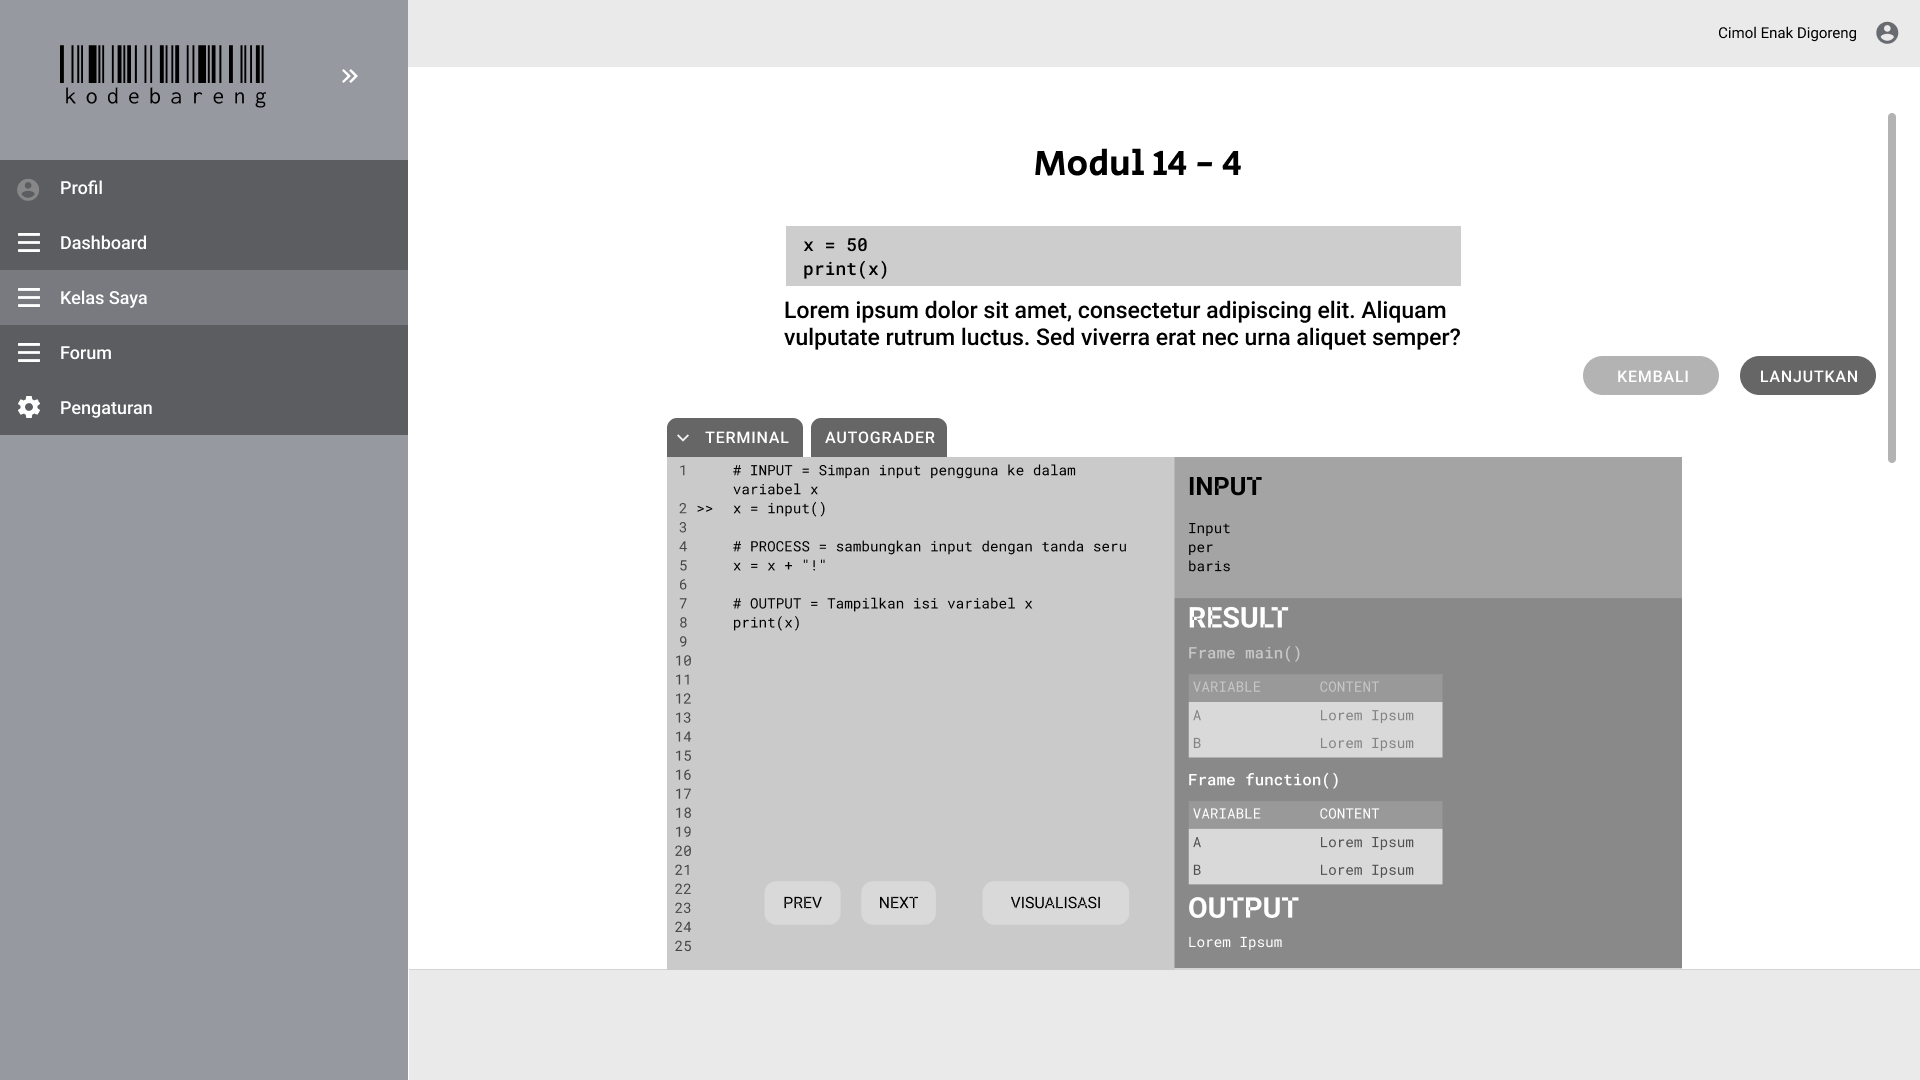
\includegraphics[width=\textwidth]{chapter3/visualizer-lesson.png}
  \caption{Wireframe Visualizer pada Lesson Stage} \label{fig:wireframe-lesson}
  Sumber: Penulis (2022)
\end{figure}

Pada sistem \textit{Backend}, ditambahkan rute baru pada \textit{Stage Controller} untuk dapat mengolah permintaan visualisasi eksekusi kode. Dibuat juga fungsi-fungsi \textit{Helper} tambahan untuk mengolah permintaan tersebut dan melanjutkannya pada sistem Autograder-Executor apabila kode diperbolehkan untuk dieksekusi.

Pada sistem \textit{Autograder-Executor}, dibuat komponen-komponen baru untuk mendapatkan informasi yang dibutuhkan untuk visualisasi. Komponen \verb|PDB (debugger)| merupakan komponen bawaan \verb|Python| yang dapat digunakan untuk melakukan \textit{debugging} pada suatu kode. Komponen \verb|Executor| digunakan untuk mengeksekusi kode program menggunakan PDB sehingga dapat dengan otomatis menjelajahi eksekusi kode program dan mendapatkan \textit{stack trace}. Komponen \verb|Parser| digunakan untuk mengolah hasil eksekusi serta \textit{stack trace} dari \verb|Executor| sehingga dapat dimanfaatkan untuk visualisasi eksekusi kode. Terdapat juga modifikasi pada Controller dan Autograder agar dapat menyesuaikan dengan spesifikasi kebutuhan fungsional. Rancangan alur kerja komponen Executor dan Parser dapat dilihat pada \autoref{fig:activity-executor}

\begin{figure}[!h]
  \centering
  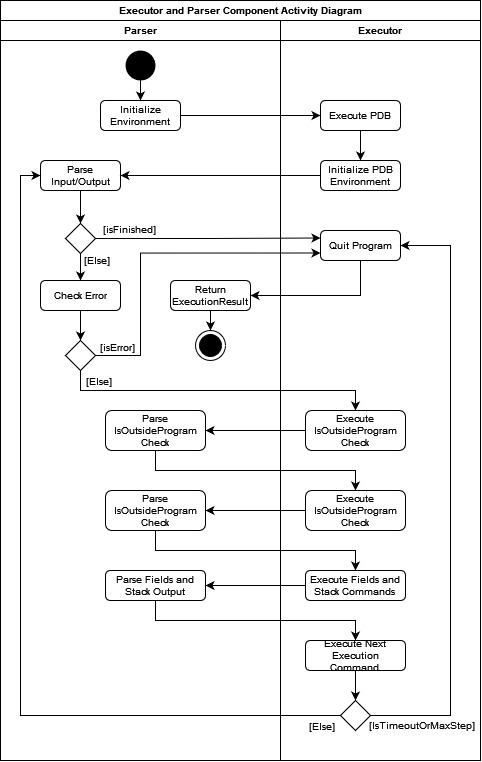
\includegraphics[width=0.9\textwidth]{chapter3/activity-executor.jpg}
  \caption{Activity Diagram Komponen Executor dan Parser} \label{fig:activity-executor}
  Sumber: Penulis (2022)
\end{figure}

Selain itu, terdapat juga fitur-fitur atau konsep dari bahasa pemrograman yang menjadi cakupan dari ILE yang dijabarkan pada \autoref{tab:ile-scope}. Cakupan ini diambil dari \textcite{moons2013pilot} dengan beberapa pengubahan agar dapat disesuaikan dengan bahasa pemrograman yang digunakan yaitu Python. Cakupan ini telah disesuaikan agar dapat mendukung materi-materi yang terdapat pada kelas Python Dasar namun tidak menutup kemungkinan dapat dikembangkan lebih lanjut agar dapat digunakan pada kelas pemrograman Python lanjut atau kelas pemrograman dengan bahasa pemrograman yang lain.

\footnotesize
\begin{longtable}[c]{|l|l|}
  \caption{Cakupan implementasi fitur bahasa pemrograman pada ILE} \label{tab:ile-scope} \\ \hline
  \rowcolor{gray!30}
  \small\textbf{Concepts}                       & \small Termasuk Implementasi?          \\ \hline
  \endfirsthead
  %
  \caption*{\autoref{tab:ile-scope} (lanjutan): Cakupan implementasi ILE}                \\ \hline
  \rowcolor{gray!30}
  \small\textbf{Concepts}                       & \small Termasuk Implementasi?          \\ \hline
  \endhead
  %
  \textbf{Input/Output}                         &                                        \\ \hline
  Standard Input/Output                         & Termasuk                               \\ \hline
  File I/O                                      & Tidak Termasuk                         \\ \hline
  \textbf{Variables}                            &                                        \\ \hline
  Variable types                                & Termasuk                               \\ \hline
  Variable scope                                & Termasuk                               \\ \hline
  Assignment of values to variables             & Termasuk                               \\ \hline
  \textbf{Selection and repetition structures}  &                                        \\ \hline
  If statement                                  & Termasuk                               \\ \hline
  While loop                                    & Termasuk                               \\ \hline
  For loop                                      & Termasuk                               \\ \hline
  \textbf{Methods}                              &                                        \\ \hline
  Method structure                              & Termasuk                               \\ \hline
  Method frames                                 & Termasuk                               \\ \hline
  Message passing                               & Termasuk                               \\ \hline
  Return values                                 & Termasuk                               \\ \hline
  Recursion                                     & Termasuk                               \\ \hline
  Lambda function                               & Tidak Termasuk                         \\ \hline
  \textbf{Arrays}                               &                                        \\ \hline
  Arrays as objects                             & Termasuk                               \\ \hline
  Array structure                               & Termasuk                               \\ \hline
  Arrays of primitives                          & Termasuk                               \\ \hline
  Arrays of references                          & Tidak Termasuk                         \\ \hline
  Array index                                   & Termasuk                               \\ \hline
  List Comprehension                            & Tidak Termasuk                         \\ \hline
  \textbf{Algorithms}                           &                                        \\ \hline
  Search algorithms                             & Tidak Termasuk                         \\ \hline
  Sort algorithms                               & Tidak Termasuk                         \\ \hline
  Data structures (linked list and binary tree) & Tidak Termasuk                         \\ \hline
  \textbf{Additional requirements}              &                                        \\ \hline
  Debugging                                     & Tidak Termasuk                         \\ \hline
  Standard libraries                            & Termasuk                               \\ \hline
\end{longtable}
\normalsize